% Created 2021-06-09 Wed 13:33
% Intended LaTeX compiler: pdflatex
\documentclass{article} [NO-DEFAULT-PACKAGES] \usepackage{wx672hyperref}
\usepackage{amsmath,amsfonts,amssymb}
\usepackage{graphicx}
\usepackage{xeCJK}
\usepackage{listings}
\author{Yuhang Ge}
\date{\today}
\title{主题模型数据分析}
\hypersetup{
 pdfauthor={Yuhang Ge},
 pdftitle={Topic model Analysis},
 pdfkeywords={},
 pdfsubject={},
 pdfcreator={Emacs 26.1 (Org mode 9.1.9)}, 
 pdflang={Cn}}
\begin{document}

% 用来设置附录中代码的样式

\lstset{
    basicstyle          =   \sffamily,          % 基本代码风格
    keywordstyle        =   \bfseries,          % 关键字风格
    commentstyle        =   \rmfamily\itshape,  % 注释的风格,斜体
    stringstyle         =   \ttfamily,  % 字符串风格
    flexiblecolumns,                % 别问为什么,加上这个
    numbers             =   left,   % 行号的位置在左边
    showspaces          =   false,  % 是否显示空格,显示了有点乱,所以不现实了
    numberstyle         =   \zihao{-5}\ttfamily,    % 行号的样式,小五号,tt等宽字体
    showstringspaces    =   false,
    captionpos          =   t,      % 这段代码的名字所呈现的位置,t指的是top上面
    frame               =   lrtb,   % 显示边框
}

\lstdefinestyle{Bash}{
    language        =   Python, % 语言选Python
    basicstyle      =   \zihao{-5}\ttfamily,
    numberstyle     =   \zihao{-5}\ttfamily,
    keywordstyle    =   \color{blue},
    keywordstyle    =   [2] \color{teal},
    stringstyle     =   \color{magenta},
    commentstyle    =   \color{red}\ttfamily,
    breaklines      =   true,   % 自动换行,建议不要写太长的行
    columns         =   fixed,  % 如果不加这一句,字间距就不固定,很丑,必须加
    basewidth       =   0.5em,
  }
  
\maketitle

\section{数据预处理}
\label{sec:org75ad168}
通过读取所有Json文件,获取每个Json数据的人物简介字段,对人物简介字段进行中文文本分词、去停用词、去数字等预处理。下面是一个样例:\\

预处理前:

\begin{quotation}
\textit{周晓文,1954年出生于北京市,中国内地导演、编剧、摄影师、制作人,毕业于北京电影学院摄影系。1986年,执导战争片《他们正年轻》,从而开启了他的导演生涯[1]。1988年,自编自导犯罪片《疯狂的代价》[2],他凭借该片获得夏威夷国际电影节荣誉奖。1991年,凭借执导的剧情片《青春无悔》获得上海大学生电影节最佳导演奖。1994年,执导剧情片《二嫫》,该片获得洛迦诺国际电影节评审团大奖[3]。1998年,执导古装宫廷剧《吕后传奇》[4]。2000年,执导古装武侠剧《天龙八部》。2002年,担任古装剧《大脚马皇后》的导演[5]。2006年,执导都市冒险剧《逃亡香格里拉》[6]。2009年,执导现代情感剧《晚婚》[7]。2011年,担任剧情片《百合》的导演和制作人,该片获得第14届电影华表奖优秀数字电影奖[8]。}
\end{quotation}

预处理后:

\begin{quotation}
\textit{周晓文\ 年出\ 生于\ 北京市\ 中国\ 内地\ 导演\ 编剧\ 摄影师\ 制作\ 毕业\ 北京电影学院摄影系\ 执导\ 战争片\ 年轻\ 开启\ 导演\ 生涯\ 自编\ 自导\ 犯罪\ 疯狂\ 代价\ 该片\ 获得\ 夏威夷\ 国际\ 电影节\ 荣誉奖\ 执导\ 剧情片\ 青春\ 无悔\ 获得\ 上海\ 大学生\ 电影节\ 最佳\ 导演奖\ 执导\ 剧情片\ 该片\ 获得\ 洛迦诺\ 国际\ 电影节\ 评审团\ 大奖\ 执导\ 古装\ 宫廷\ 吕后\ 传奇\ 执导\ 古装\ 武侠剧\ 天龙八部\ 担任\ 古装剧\ 大脚\ 马皇后\ 导演\ 执导\ 都市\ 冒险\ 逃亡\ 香格里拉\ 执导\ 现代\ 情感\ 晚婚\ 担任\ 剧情片\ 百合\ 导演\ 制作\ 该片\ 获得\ 电影\ 华表奖\ 优秀\ 数字\ 电影}
\end{quotation}

\section{LDA主题模型分析}
\label{sec:org56904e1}

\subsection{最优主题数寻找}

通过分别计算区间$K=\{2-40\}$内主题的主题一致性(coherence value),绘制出下图,可以找到最优主题数为$k=6$。

\begin{center}
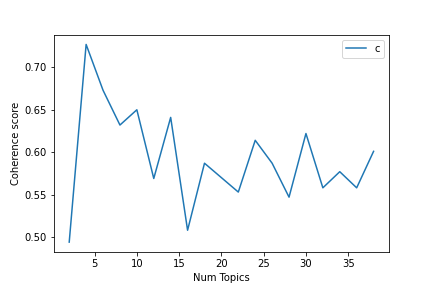
\includegraphics[width=1.0\linewidth]{./static/coherence.png}
\end{center}  

将处理后的数据通过LDA主题模型进行数据分析,设置最优主题数为6,并且每个主题的主题词数为20,得到主题分布如下:\\

\begin{quotation}
(0,
  '0.025*"主演" + 0.018*"出演" + 0.016*"电视剧" + 0.015*"饰演" + 0.012*"电影" + '
  '0.010*"获得" + 0.010*"中国" + 0.009*"生于" + 0.008*"同年" + 0.007*"参演" + 0.006*"古装" '
  '+ 0.006*"毕业" + 0.006*"日出" + 0.006*"都市" + 0.005*"最佳" + 0.005*"参加" + '
  '0.005*"个人" + 0.005*"内地" + 0.005*"情感" + 0.005*"爱情"'),
  
 (1,
  '0.027*"主演" + 0.026*"电影" + 0.016*"获得" + 0.015*"中国" + 0.011*"最佳" + '
  '0.009*"电视剧" + 0.008*"生于" + 0.007*"执导" + 0.007*"出演" + 0.007*"饰演" + '
  '0.006*"同年" + 0.006*"电影节" + 0.005*"参演" + 0.005*"导演" + 0.005*"爱情" + '
  '0.005*"担任" + 0.005*"上映" + 0.005*"日出" + 0.005*"毕业" + 0.004*"公主"'),
  
 (2,
  '0.015*"中国" + 0.012*"获得" + 0.011*"专辑" + 0.008*"发行" + 0.007*"电视剧" + '
  '0.007*"生于" + 0.006*"最佳" + 0.006*"主演" + 0.006*"电影" + 0.006*"音乐" + 0.005*"同年" '
  '+ 0.005*"演员" + 0.005*"公元前" + 0.005*"参加" + 0.005*"日出" + 0.004*"出演" + '
  '0.004*"担任" + 0.004*"成为" + 0.004*"推出" + 0.003*"个人"'),
  
 (3,
  '0.011*"中国" + 0.010*"获得" + 0.008*"主演" + 0.006*"生于" + 0.005*"皇后" + 0.005*"电影" '
  '+ 0.005*"最佳" + 0.005*"电视剧" + 0.004*"韩国" + 0.004*"出演" + 0.004*"担任" + '
  '0.004*"皇帝" + 0.004*"元年" + 0.003*"导演" + 0.003*"时期" + 0.003*"日本" + 0.003*"爱情" '
  '+ 0.003*"大赏" + 0.003*"日出" + 0.003*"女演员"'),
  
 (4,
  '0.022*"电影" + 0.010*"出演" + 0.009*"参演" + 0.009*"饰演" + 0.008*"生于" + 0.007*"中国" '
  '+ 0.007*"主演" + 0.007*"获得" + 0.007*"最佳" + 0.007*"香港" + 0.006*"电视剧" + '
  '0.005*"演员" + 0.005*"执导" + 0.004*"日出" + 0.004*"时期" + 0.004*"成为" + 0.003*"导演" '
  '+ 0.003*"谥号" + 0.003*"毕业" + 0.003*"大臣"'),
  
 (5,
  '0.017*"电影" + 0.012*"获得" + 0.011*"最佳" + 0.010*"中国" + 0.009*"主演" + 0.009*"生于" '
  '+ 0.006*"香港" + 0.006*"演员" + 0.005*"同年" + 0.005*"参演" + 0.005*"个人" + '
  '0.004*"台湾" + 0.004*"日出" + 0.004*"电视剧" + 0.004*"毕业" + 0.004*"成为" + '
  '0.004*"专辑" + 0.004*"音乐" + 0.003*"出演" + 0.003*"男演员"')
\end{quotation}

\section{主题可视化}
\label{sec:orgdb08b28}

下面是分别6个主题分布的可视化图:\\

主题1:

\begin{center}
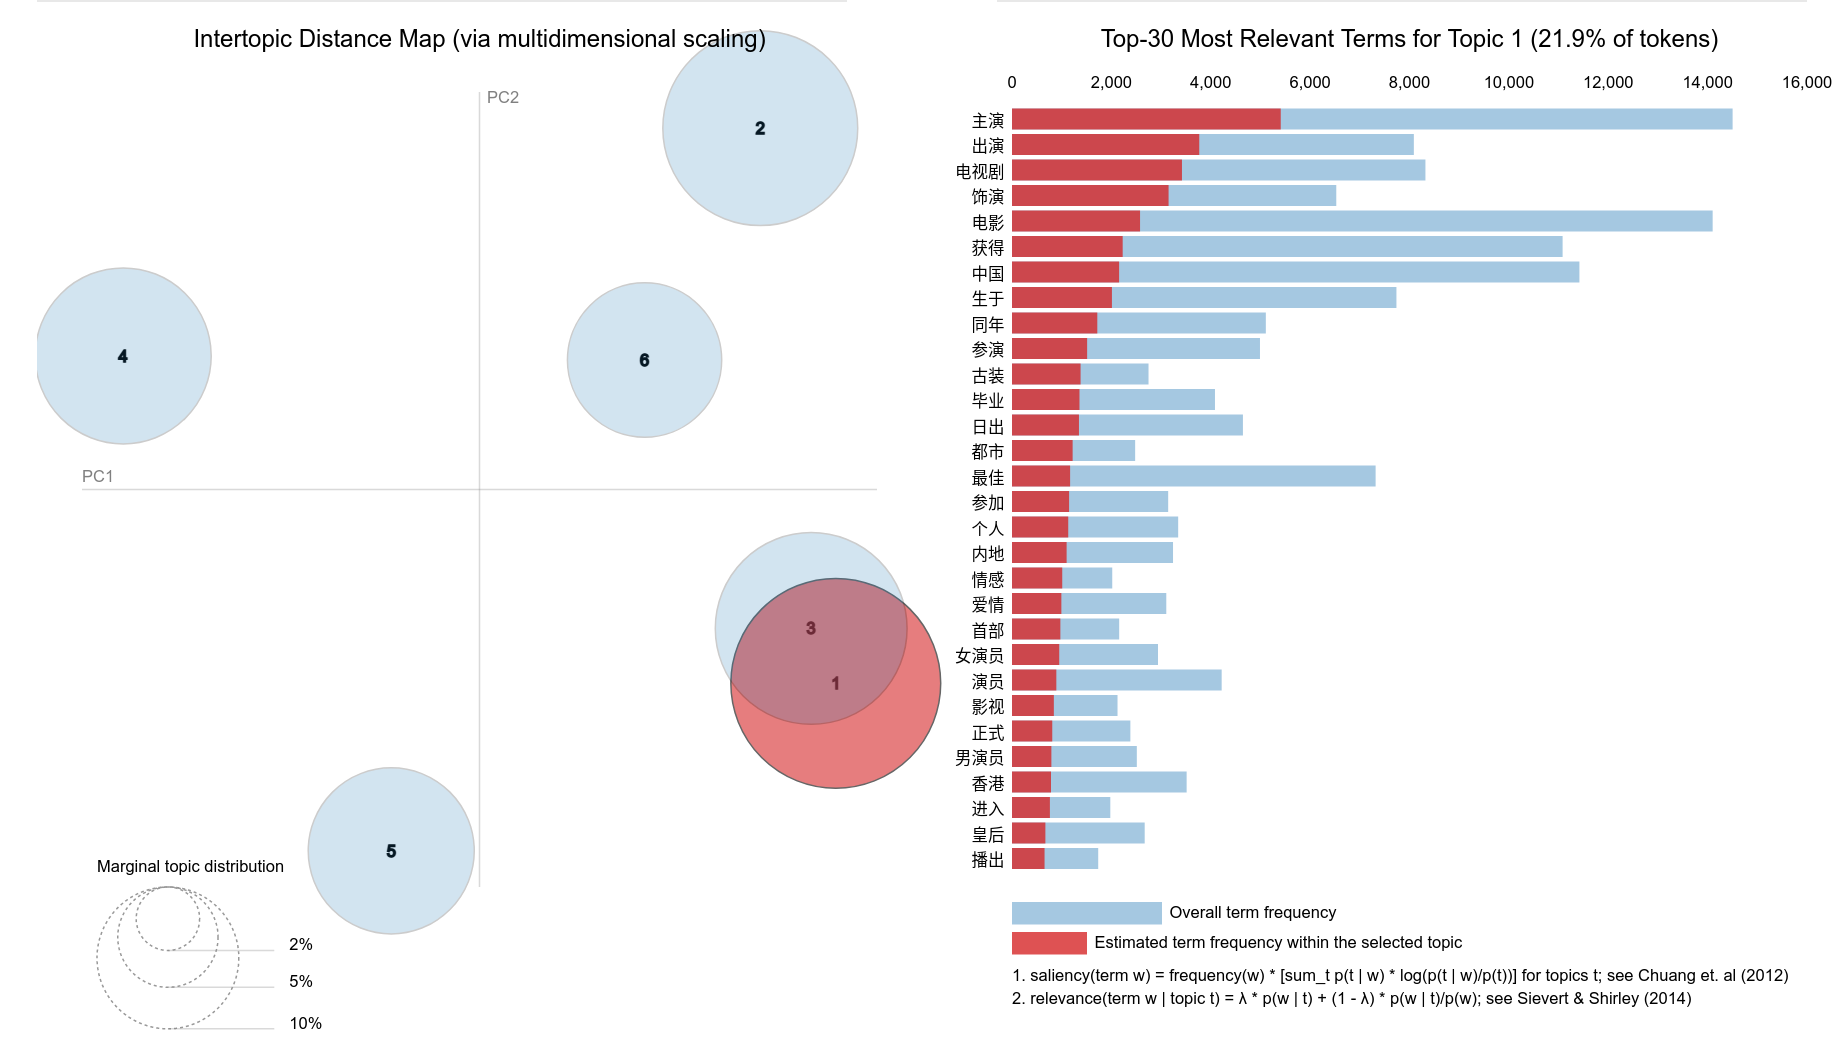
\includegraphics[width=1.0\linewidth]{./static/topic-vis-01.png}
\end{center}

主题2:

\begin{center}
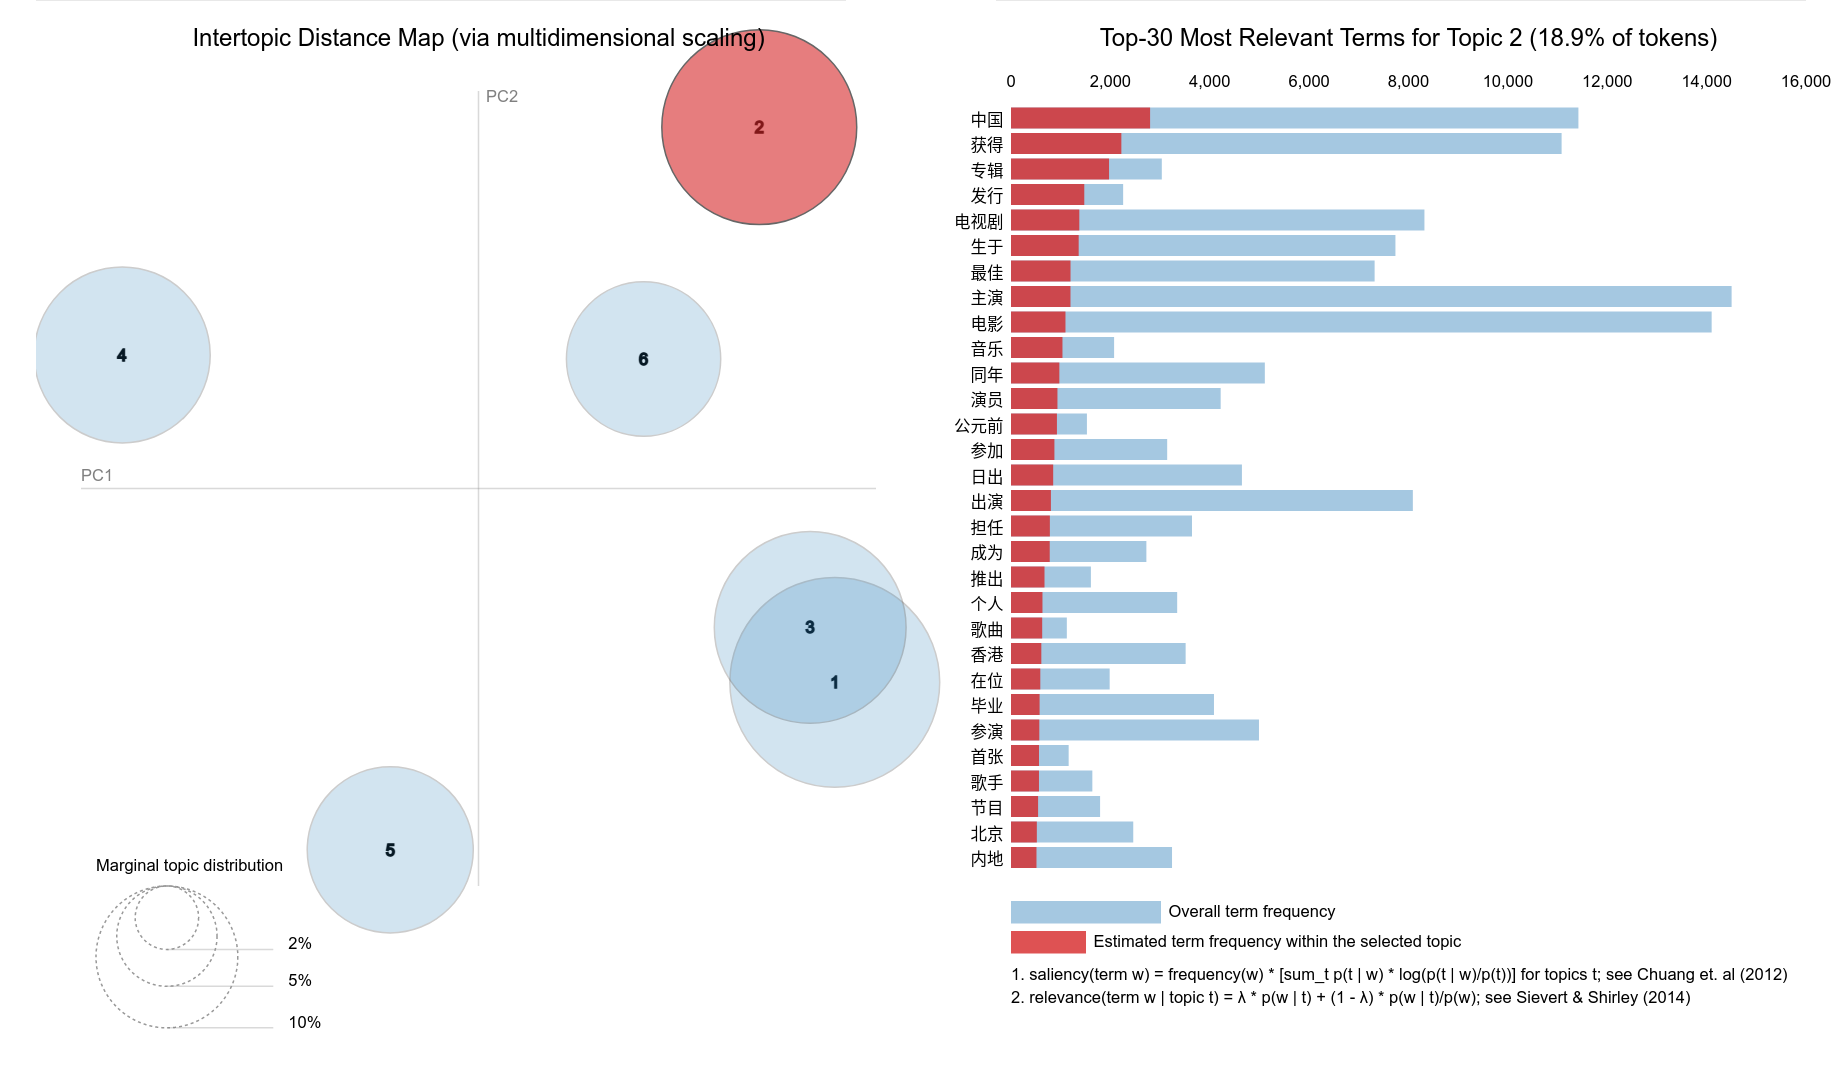
\includegraphics[width=1.0\linewidth]{./static/topic-vis-02.png}
\end{center}  

主题3:

\begin{center}
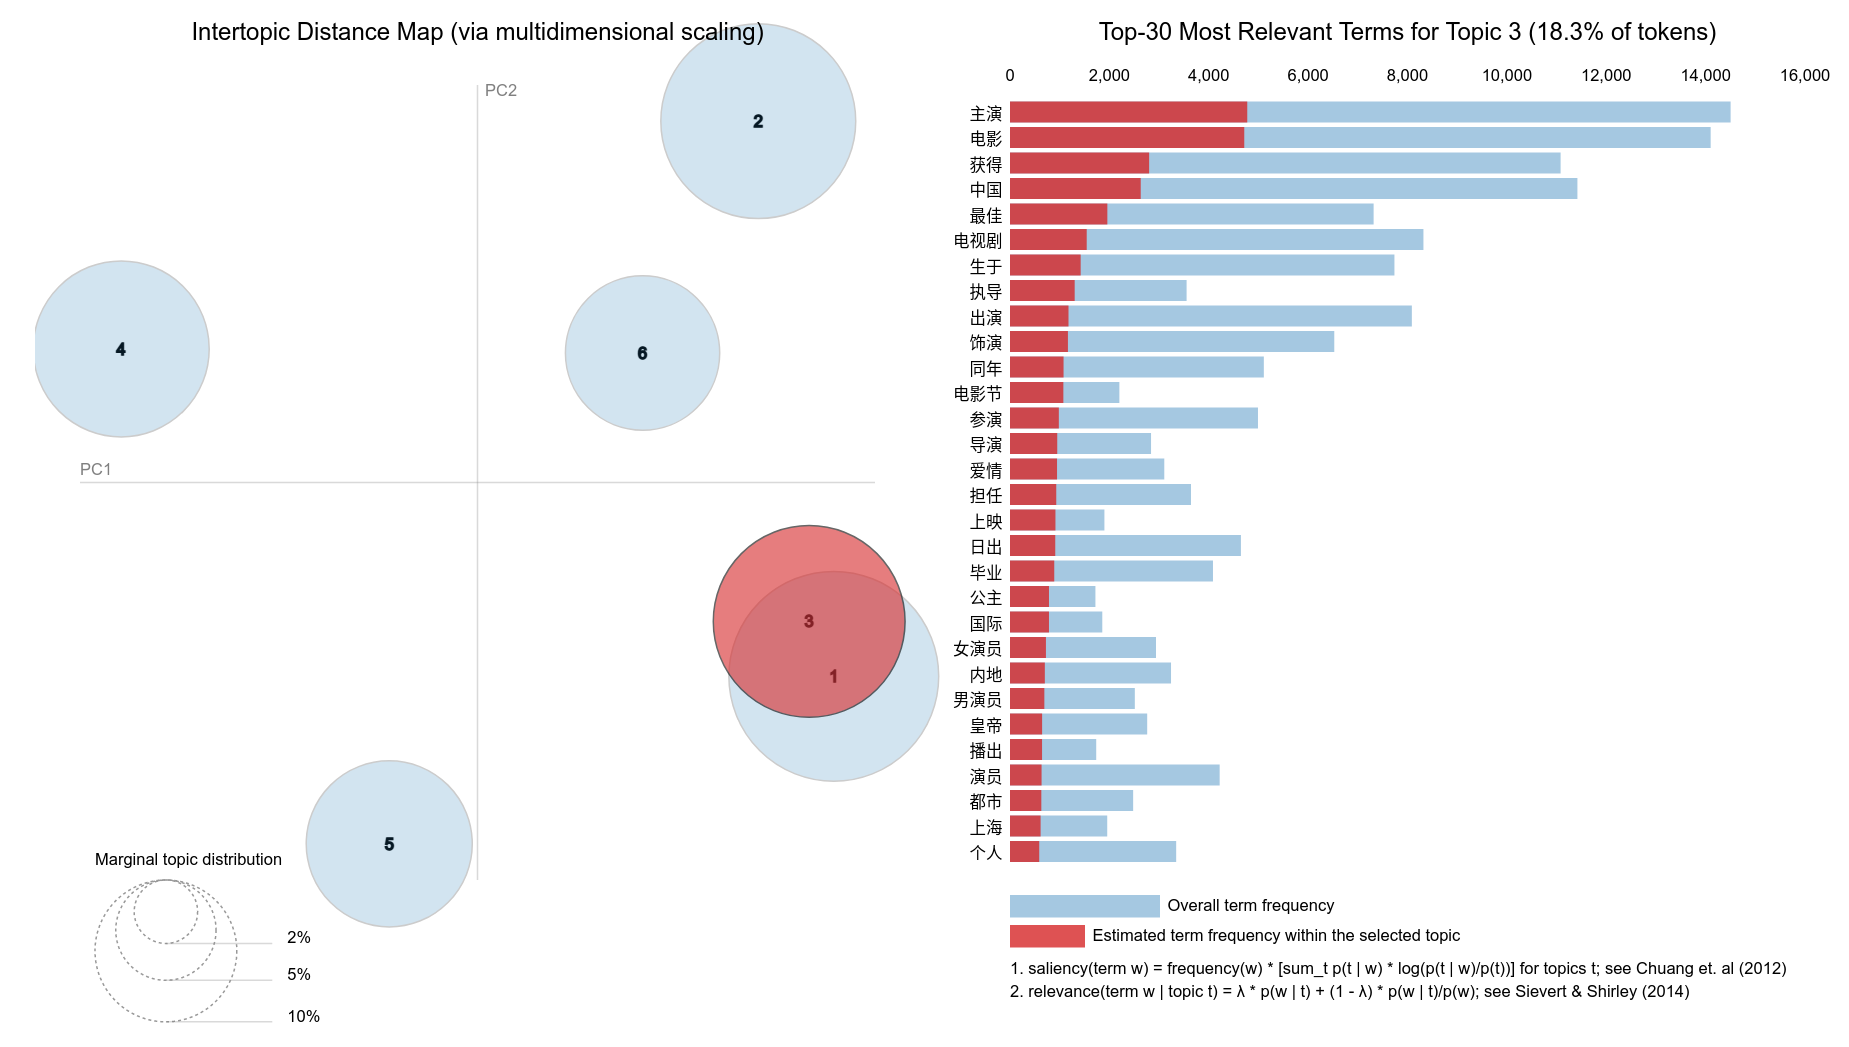
\includegraphics[width=1.0\linewidth]{./static/topic-vis-03.png}
\end{center}

主题4:

\begin{center}
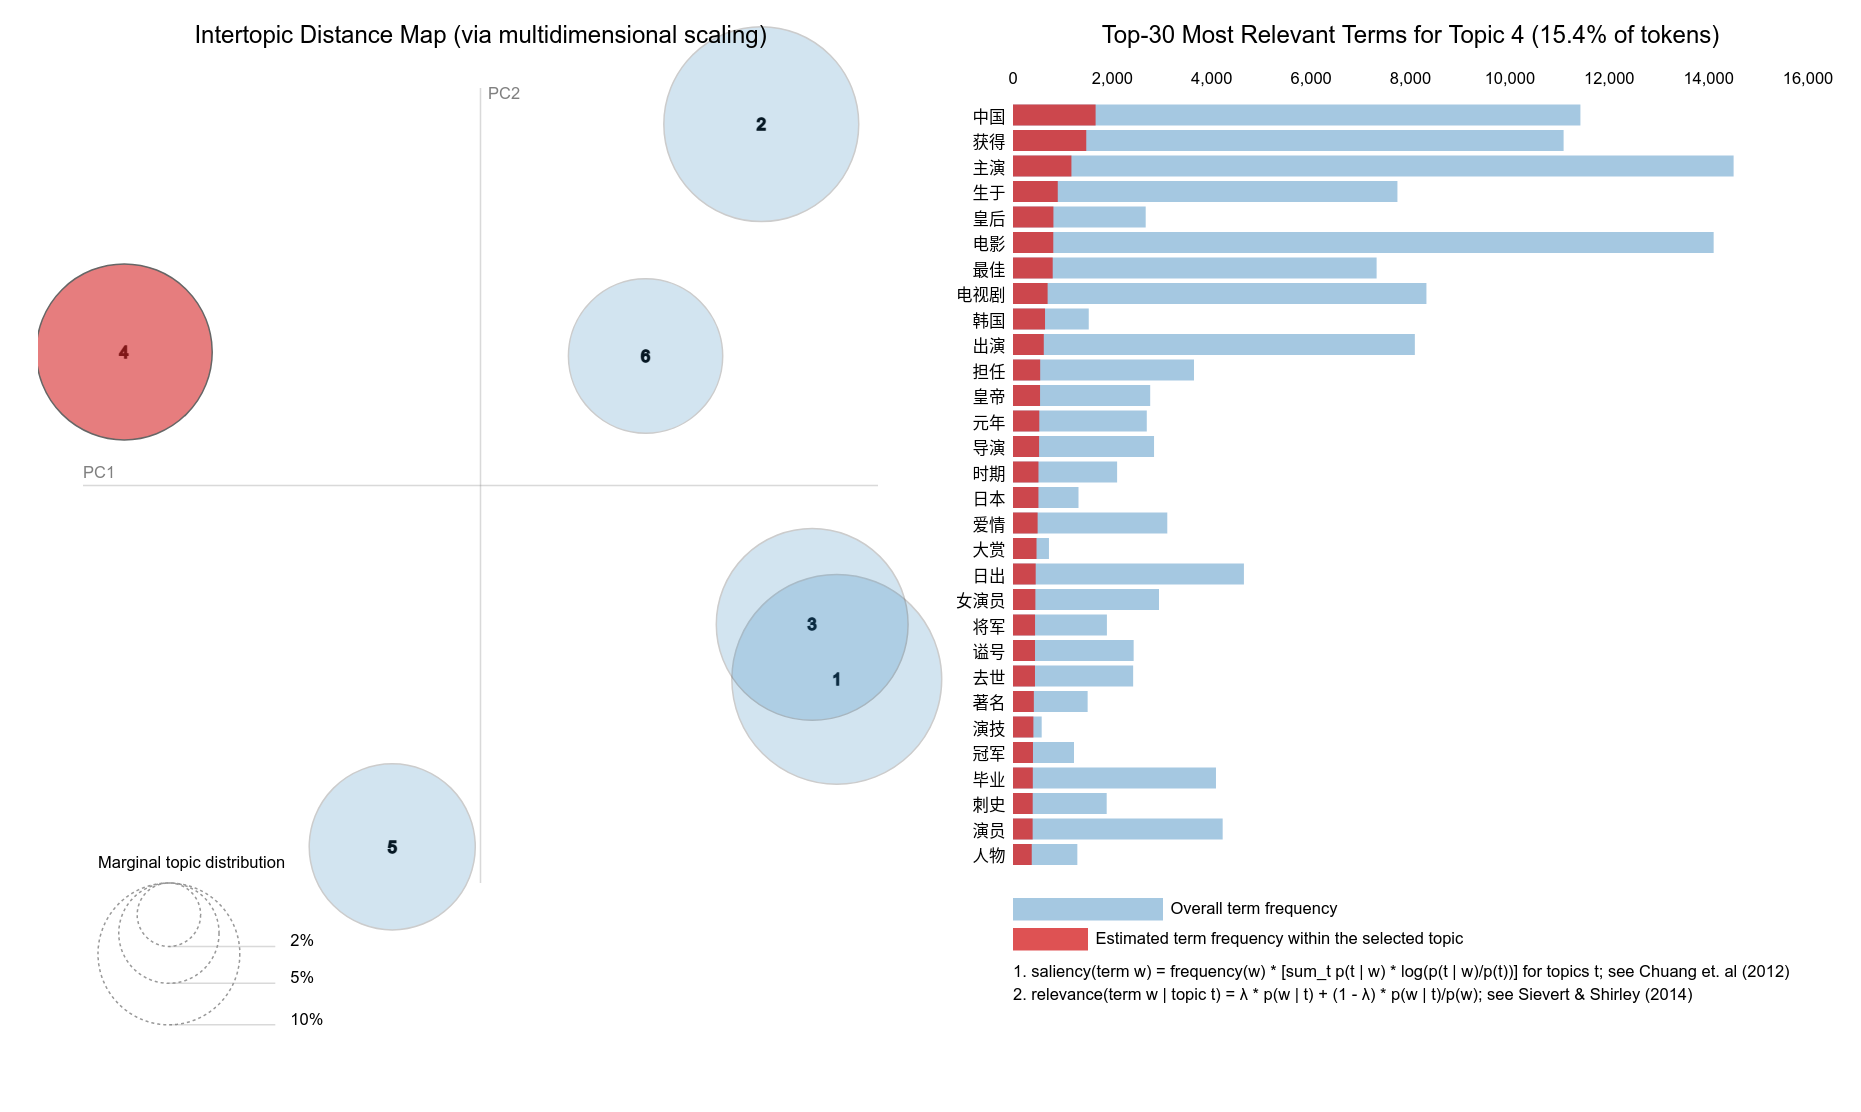
\includegraphics[width=1.0\linewidth]{./static/topic-vis-04.png}
\end{center}  

主题5:

\begin{center}
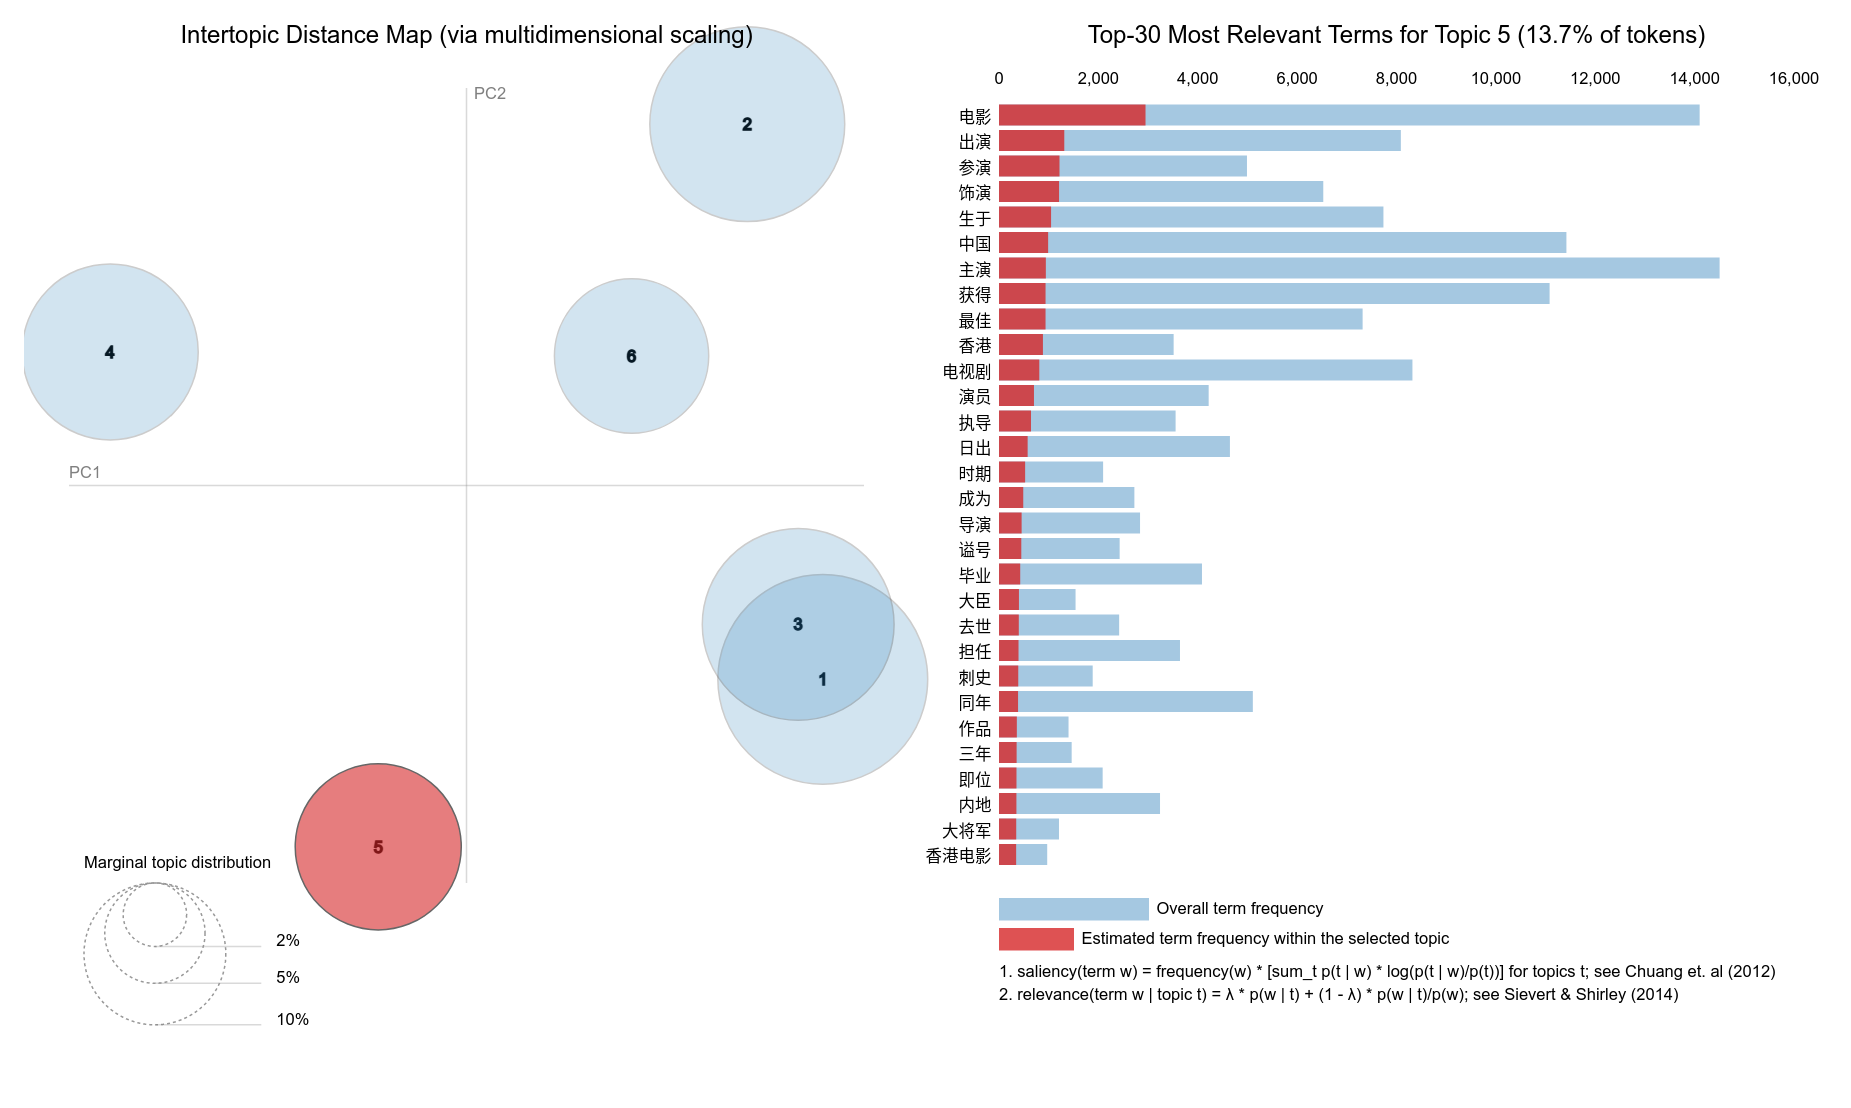
\includegraphics[width=1.0\linewidth]{./static/topic-vis-05.png}
\end{center}  

主题6:

\begin{center}
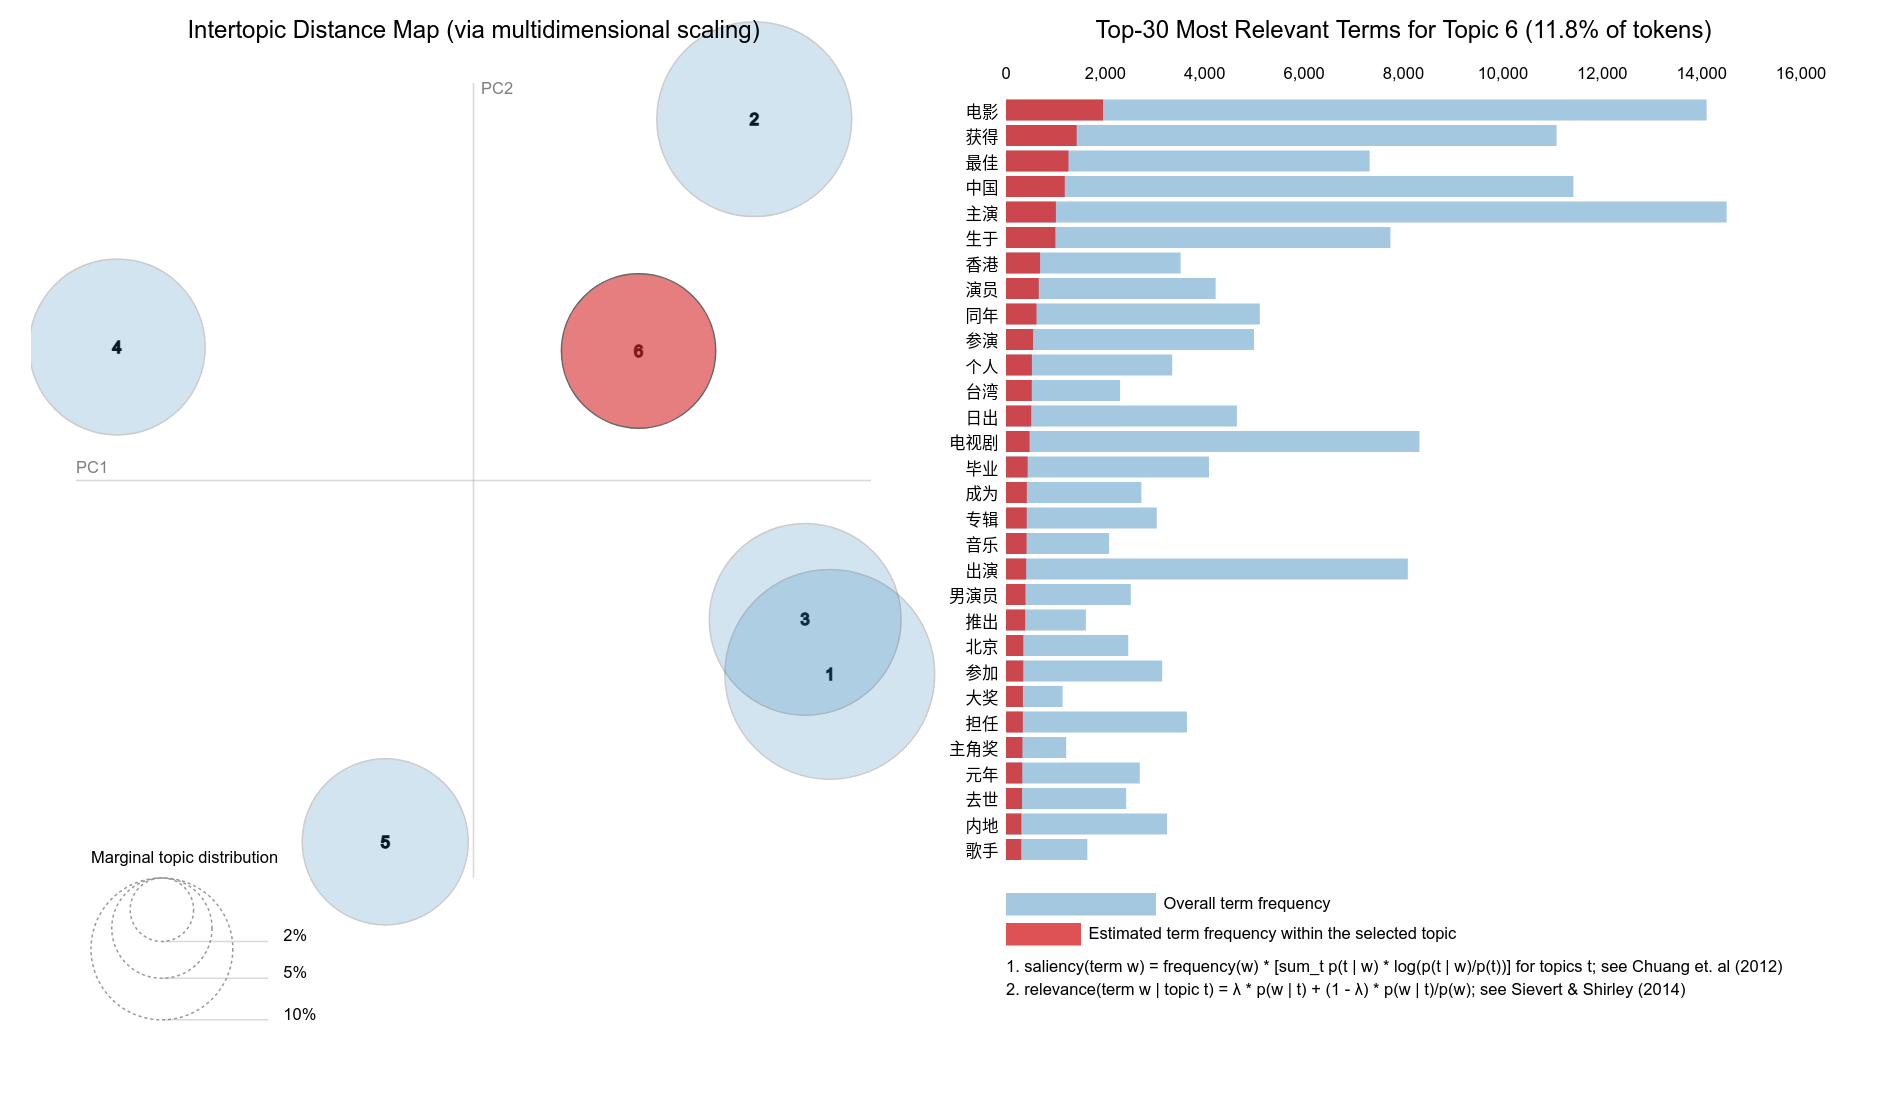
\includegraphics[width=1.0\linewidth]{./static/topic-vis-06.png}
\end{center}  

\end{document}